\epigraph{
"Yields falsehood when \\ preceded by its quotation" \\
yields falsehood when \\ preceded by its quotation
}{
Quine's paradox
}


This chapter describes an implementation of \algo that uses
Nested Data Parallelism in Haskell (as in \cite{Harness2008}).
First, a few predefined functions are presented to
increase their the understanding of their operational behaviour.
Then the implementation is presented
and finally its complexities are calculated.

\section{Utilities}

  \subsection*{Scanl}
    Parallel prefix sum has well studied efficient implementations.
    One of them is the following:
    \begin{lstlisting}   
scanlP f z xs =
joinD
. mapD (\(as,a) -> mapS (f a) as)
. propagateD f z
. mapD (scanlS f z)
. splitD
$ xs
    \end{lstlisting}
    This implementation is designed to reduce communication
    and therefore increase efficiency. It works in three steps.
    First, each PU computes its local prefix sum (line 5).
    Second, the total sum of each of the PUs is propagated
    - adding up subsequent values (line 4).
    Third, the updated sum is used to increase the values of the local chunks (line 39).
    This approach is visualised in figure \ref{figure:scanlPsteps}
    
    \begin{figure}[h!]
        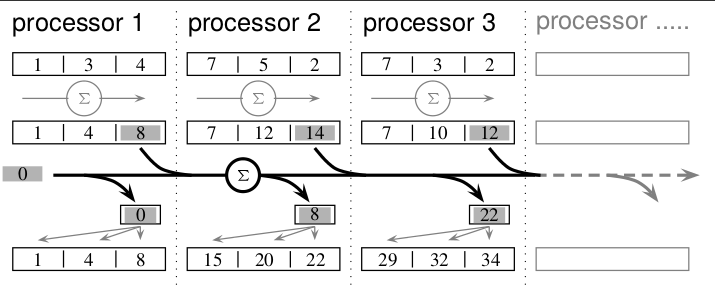
\includegraphics[width=\linewidth]{scanlP-three-steps.png}
        \caption[Three-Step Parallel Prefix Sum]{Parallel prefix sum in three steps (Figure from \cite{DistTypes1999}) }
        \label{figure:scanlPsteps}
    \end{figure}
    In terms of depth and parallel complexity, the propagation is the bottleneck.
    However, since the propagation itself is structurally isomorphic to prefix summing itself,
    one can use a binary-tree-like scheme for propagation for the local values distributed on the PUs.
    This propagation runs in time logarithmic to the number of PUs.
    It an be derived from \cite{Scanl1980}. For the purposes of this thesis,
    it is sufficient to state the following complexities for \c{scanlP (+) 0}:
    $\W(n) \in O(n)$ and $\D(n) \in O(\log n)$.

  \subsection*{GroupP}
    \c{groupP} is a frequently used function in functional programming.
    It's type is \type{[:a:] -> [:[:a:]:]} and given an array it returns an array of arrays,
    where each subarray contains equal consecutive
    elements of the source array. For example
    \c{groupP [4,2,2,2,2,3,3,1]} becomes \c{[[4],[2,2,2,2],[3,3],[1]]}.
    In NDP, the latter is represented by
    \begin{lstlisting}
AArr {
  data = [# 4,2,2,2,3,3,1 #],
  indices = [# 0,1,5,7 #]
  lengths = [# 1,4,2,1 #]
}
    \end{lstlisting}
    An efficient parallel implementation of \c{groupP}
    relies on the following key insight: The \c{data} field in the nested array
    is the identical to the source array itself. To implement \c{groupP} one only
    needs to efficiently calculate the segment descriptor field
    and attach it to the source array. This is
    possible in depth logarithmic to the size of the input array.
    
    \begin{figure}[h!]
        \begin{center}
        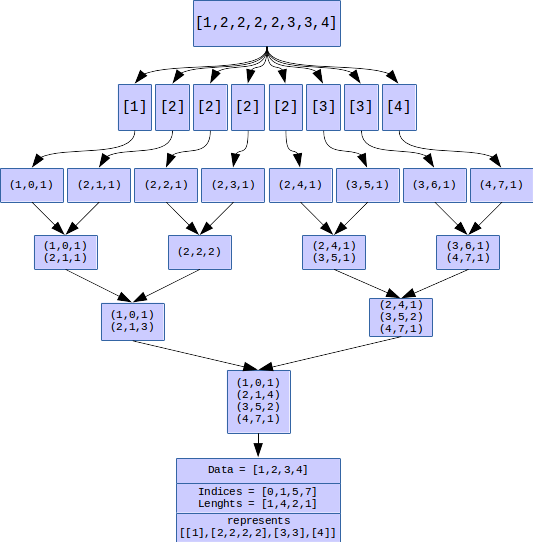
\includegraphics[width=\linewidth]{groupP.png}
        \caption[Parallel Evaluation of \c{groupP}]{An example calculation of groupP. Each box is a PU.}
        \label{figure:groupP}
        \end{center}
    \end{figure}
    
    As visualised in the figure \ref{figure:groupP},
    all elements are split onto the PUs first.
    Then each PU creates a local chunk of a linked list of
    \c{(Value,StartIdx,Count)}-Triplets to record its singleton.
    After that, each level of recursion merges two PUs by
    merging the last triplet of the left list with the first triplet
    of the right list. If both triplets correspond to the same value,
    then a new triplet with the total count and the left index is used.
    If both are unequal, then they are left unchanged. The implementation
    of \c{groupP} uses a sub-function \c{segdSplitMerge} to implement the
    splitting and merging. This function will be exposed later-on in
    the vectorization of \ndpn.
    Further analysis reveals the complexities $\W(n) \in O(n)$ and $\D(n) \in O(\log n)$.
    All in all, \c{groupP} is an operation which can very well exploit the flat representation of nested arrays.
    % NO DO: and to appendix and refer to it?
    
  \subsection*{SortP}
    General parallel sorting can be as simple as a parallel
    implementation of merge-sort \cite{ParMergeSort1988} where the recursive calls are executed
    in parallel. \c{sortP} of type \type{[:Int:] -> [:Int:]} implements this,
    and has complexities of $\W(n) \in O(n \log n)$
    and $\D(n) \in O(\log n)$.
    \footnote{There exists other sorting mechanism
    like \emph{Batcher's Bitonic Sort} \cite{BitonicSort1968} with $O(n \log^2 n)$ work and $O(\log^2 n)$
    depth. The author did not use its implementation as it is sophisticated and
    the workload of its vectorization were expected to be enormous (on top of the all the other work).
    Retrospectively, the thesis does not inline and expose the internals of \c{sortP} in \ndpv.
    But this was not clear beforehand.
    }

  \subsection*{Histogram calculation}
    Conventional functional programming often enables one to write
    consise and correct implementations by composing
    independent and general functions. For example -
    consider the problem of run length encoding. Given a (possibly long) array,
    the goal is to create a sparse array that compresses elements
    by encoding consecutive equal elements
    with a tuple of the element and its number of occurrences.
    E.g. it transforms \c{[4,2,2,2,2,3,3,1]} to \c{[(4,1),(2,4),(3,2),(1,1)]}.
    An implementation can be formulated directly.
    \begin{lstlisting}
runLengthEncode :: [:a:] -> [:(a,Int):]
runLengthEncode = mapP (\xs -> (headP xs, lengthP xs)) . groupP
    \end{lstlisting}
    This function uses \c{groupP} to first create sub-arrays of
    equal consecutive elements. Then it
    transforms sub-arrays like \c{[2,2,2,2]} to tuples like \c{(2,4)}.
    This is the second step of run length encoding.
    
    Run length encoding is an useful intermediate step in
    creating the histogram. It implements the "counting"-property
    of a histogram.
    To make create a full histogram, the input image has to be flattened first (\¢{unconcatP}),
    then sorted(\c{sortP}) and finally applied \c{runLengthEncode} on.
    The sorting is necessary, as it groups together pixels regardless of their
    position in the original image.
    The result is an array of type \type{[:(Int,Int):]} where each element
    describes a gray tone (first integer in tuple) and its number of
    occurrences (second integer in tuple).
    Using this approach, one has a parallel implementation of the histogram calculation.
    Comping up with this approach is easier than creating an entire
    reduction as was the case in \man.
    
\section{Implementation}
  One can now give the implementation of \ndpn. The code
  implements \algo using Nested Data Parallelism in Haskell
  and is given below:
  \begin{lstlisting}
type Image = [:[:Int:]:]
type Hist a = [:a:]

hbalance :: Image -> Image
hbalance img =
  let h = hist img
      a = accu h
      a0 = headP a
      agmax = lastP a
      n = normalize a0 agmax a
      gs = scale gmax n
      img' = apply gs img
  in  img'

hist :: Image -> Hist Int
hist = sparseToDenseP (gmax+1) 0
        . mapP (\g -> (headP g,lengthP g))
        . groupP
        . sortP
        . concatP

accu :: Hist Int -> Hist Int
accu = scanlP (+) 0

normalize :: Int -> Int -> Hist Int -> Hist Double
normalize a0' agmax' as =
  let a0 = fromIntegral a0'
      agmax = fromIntegral agmax'
      divisor = agmax - a0
  in  mapP ( \freq' -> (fromIntegral freq' - a0) / divisor ) as

scale :: Int -> Hist Double -> Hist Int
scale gmax as = mapP ( \a -> floor (a * fromIntegral gmax) ) as

apply :: Hist Int -> Image -> Image
apply as img = mapP (mapP (as !:)) img
  \end{lstlisting}
  The first two lines describe the data structure used to encode an image - 
  namely nested data-parallel arrays.
  As described in the basics chapter - in NDP
  nested arrays are converted to flat data and a segment descriptor
  during vectorization. Therefore nesting
  can be used from the programmer point of view to simplify
  the programming and to support the intuition - without
  sacrificing performance.
  
  \ndpn, like the description of \algo, 
  is split up in histogram calculation (lines 20 - 16)
  ,histogram accumulation (line 23), normalisation (lines 26 - 30),
  scaling (line 33) and the final gray tone mapping (line 36).
  The significant different between \ndpn and \seq is the calculation of the histogram.
  \footnote{Aside from the the less significant fact, that \ndpn uses an array for its histogram while \seq uses a binary-search-tree.}
  In \ndpn, it is implemented based on the approach explained in the
  previous section. First, it flattens the array, then it sorts it and afterwards
  it uses run length encoding.
  
  At the end, however, it uses \c{sparseToDenseP}\footnote{Its type is  \type{Int -> a -> PA (Int,a) -> PA a}}.
  The expression \c{sparseToDenseP size z} to converts the sparse array (typed \type{[:(Int,Int):]})
  to its corresponding dense array (typed \type{[:Int:]}).
  The dense array has size \c{size} and inserts \c{z} for elements not specified in the sparse array
  \footnote{E.g. \c{ sparseToDenseP 8 0 [: (1,5),(2,4),(6,7) :] => [: 0,5,4,0,0,0,7,0 :]}}
  .
  Using this approach, \c{hist} can create an array where
  the element at the index \c{i} is the number of occurrences
  of the gray tone \c{i} in the original image.
  This is a simpler format for the histogram.
  \footnote{Keeping sparse arrays for the representation of the histogram is a viable option yielding possibly different (maybe better?) complexities.}
  
  The function \c{apply} uses a nested application of parallel functions.
  Within NDP, it will be subject to flattening in \ndpv.
  
\section{Complexities}
  Using the work and depth measures as introduced in section \ref{section:parmeasures},
  one can assign the following measures to the functions involved.
  Let $n$ be the number of pixels in an $w \times h$ image,
  then the complexities are given in table \ref{complexities:ndpn}.
  \begin{table}[h!]
    \caption{Complexities for \ndpn}
    \label{complexities:ndpn}
    \begin{center}
    \begin{tabular}{lll}
        \toprule
        function or variable & $\W \in O(...)$           & $\D \in O(...)$ \\
        \midrule
        hbalance        & $n \log n + gmax$   & $\log n + \log gmax$\\
        \midrule
        hist            & $n \log n + gmax$    & $\log$ n \\
        sparseToDenseP  & gmax                 & 1 \\
        groupP          & n                    & $\log$ n \\
        sortP           & n $\log$ n             & $\log$ n \\
        concatP         & 1                    & 1 \\
        \midrule
        accu            & gmax                 & $\log$ gmax \\
        scanlP          & gmax                 & $\log$ gmax \\
        \midrule
        normalize       & gmax                 & 1 \\
        scale           & gmax                 & 1 \\
        \midrule
        apply           & $n = w \cdot h$ & 1 \\
    \end{tabular}
    \end{center}
  \end{table}
    For the depths, \c{hist} and \c{accu} get logarithmic bounds by
    either the size of the image and the maximum gray tone, respectively.
    All in all, \ndpn has $\W \in O(n \log n + gmax)$
    and $\D \in O(\log n + \log gmax)$.
    
    \ndpn is mostly a direct translation of \seq and \algo.
    A parallel implementation of histogram calculation is given
    by using only common purely functional processing operations (such as \c{grouP} and \c{sortP}).
    All in all, it involves less workload for the programer then it was
    the case in \man.
    
    
    In the next chapter \ndpn is going to be transformed into \ndpv
    manually. It will show, what the compiler would do automatically.
  
  
